% arara: lualatex: { shell : yes }
% arara: lualatex: { shell : yes }

\documentclass[a4paper,11pt]{kth-mag}
\DeclareMathSizes{12}{}{}{}

% Math and code packages
\usepackage{amsmath}   % all things math
\usepackage{amssymb}   % additional math symbols
\usepackage{xfrac}     % nice fractions in body of text
\usepackage{siunitx}   % typesets numbers with units
\usepackage{mathtools} % extensions for amsmath
\usepackage[section]{minted}    % advanced code examples

% Tables
\usepackage{booktabs} % professionally looking tables
\usepackage{tabulary} % whole page tables

% Caption and split floats
\usepackage{caption}    % customizable captions
\usepackage{subcaption} % nice subfigures and subtables

% Bibliographies
\usepackage[backend=biber]{biblatex} % modern bibliographies

% PDF Metadata
\usepackage{hyperref} % enables PDF hyperlinks

% Fonts, typography and languages
\usepackage{fontspec}     % all things fonts
\defaultfontfeatures{Ligatures=TeX}
\setmainfont{FiraSans-Book.otf}[
  BoldFont = FiraSans-SemiBold.otf,
  ItalicFont = FiraSans-Italic.otf,
  BoldItalicFont = FiraSans-SemiBoldItalic.otf]
\setsansfont{FiraSans-Regular.otf}[Scale=MatchLowercase]
\setmonofont{FiraMono-Regular.otf}[Scale=MatchLowercase]
\usepackage{unicode-math} % use custom fonts for math
\setmathfont{Asana-Math.otf}
\usepackage{microtype}	  % advanced typesetting
\DisableLigatures{family=tt*}
\usepackage[main=english, swedish]{babel} % language-specific conventions

% Graphics
\usepackage{graphicx} % all things graphics
\usepackage{pgfplots} % complex graphs
\usepackage{pgfplotstable}
\pgfplotsset{
  compat=1.11, % avoid running in backwards compatibility mode
  width=\textwidth,
  tick label style = {font=\ttfamily},
  every axis label = {font=\sffamily},
  legend style = {font=\sffamily},
  label style = {font=\sffamily},
  separate axis lines,
  y axis line style={draw opacity=0},
  x axis line style={gray},
  axis x line*=bottom,
  axis y line*=left,
  major tick length=0pt,
  grid=both,
  y grid style={dashed},
  legend pos=north west,
}
\definecolor{set11}{RGB}{228,  26,  28}
\definecolor{set12}{RGB}{ 55, 126, 184}
\definecolor{set13}{RGB}{ 77, 175,  74}
\definecolor{set14}{RGB}{152,  78, 163}
\definecolor{set15}{RGB}{255, 127,   0}
\definecolor{set16}{RGB}{255, 255,  51}
\definecolor{set17}{RGB}{166,  86,  40}
\definecolor{set18}{RGB}{247, 129, 191}
\definecolor{set19}{RGB}{153, 153, 153}

\definecolor{set11_light}{RGB}{251, 180, 174}
\definecolor{set12_light}{RGB}{179, 205, 227}
\definecolor{set13_light}{RGB}{204, 235, 197}
\definecolor{set14_light}{RGB}{222, 203, 228}
\definecolor{set15_light}{RGB}{254, 217, 166}
\definecolor{set16_light}{RGB}{255, 255, 204}
\definecolor{set17_light}{RGB}{229, 216, 189}
\definecolor{set18_light}{RGB}{253, 218, 236}
\definecolor{set19_light}{RGB}{242, 242, 242}

% \definecolor{set11}{cmyk}{.1 ,.9 ,.8 ,.0 }
% \definecolor{set12}{cmyk}{.8 ,.3 ,.0 ,.0 }
% \definecolor{set13}{cmyk}{.7 ,.0 ,.8 ,.0 }
% \definecolor{set14}{cmyk}{.4 ,.65,.0 ,.0 }
% \definecolor{set15}{cmyk}{.0 ,.5 ,1.0,.0 }
% \definecolor{set16}{cmyk}{.0 ,.0 ,.8 ,.0 }
% \definecolor{set17}{cmyk}{.35,.6 ,.8 ,.0 }
% \definecolor{set18}{cmyk}{.0 ,.5 ,.0 ,.0 }
% \definecolor{set19}{cmyk}{.0 ,.0 ,.0 ,.4 }
%
% \definecolor{set11_light}{cmyk}{.0 ,.3 ,.2 ,.0 }
% \definecolor{set12_light}{cmyk}{.3 ,.1 ,.0 ,.0 }
% \definecolor{set13_light}{cmyk}{.2 ,.0 ,.2 ,.0 }
% \definecolor{set14_light}{cmyk}{.12 ,.17,.0 ,.0 }
% \definecolor{set15_light}{cmyk}{.0 ,.15 ,.3,.0 }
% \definecolor{set16_light}{cmyk}{.0 ,.0 ,.2 ,.0 }
% \definecolor{set17_light}{cmyk}{.1,.12 ,.2 ,.0 }
% \definecolor{set18_light}{cmyk}{.0 ,.15 ,.0 ,.0 }
% \definecolor{set19_light}{cmyk}{.0 ,.0 ,.0 ,.05 }

\usepackage{modifications}

\linespread{1.2}

\title{GPU Simulation of Rigid Fibers}

\foreigntitle{GPU simulering av stela fibrer}

\author{Eric Wolter}
\date{January 2015}
\blurb{Master's Thesis at School of Engineering Sciences\\Supervisor: Katarina Gustavsson\\Examiner: Michael Hanke}
\trita{TRITA xxx yyyy-nn}

\begin{document}
\frontmatter
\pagestyle{empty}

\maketitle
\selectlanguage{english}
\begin{abstract}
Lorem ipsum dolor sit amet, consectetuer adipiscing elit. Mauris
purus. Fusce tempor. Nulla facilisi. Sed at turpis. Phasellus eu
ipsum. Nam porttitor laoreet nulla. Phasellus massa massa, auctor
rutrum, vehicula ut, porttitor a, massa. Pellentesque fringilla. Duis
nibh risus, venenatis ac, tempor sed, vestibulum at, tellus. Class
aptent taciti sociosqu ad litora torquent per conubia nostra, per
inceptos hymenaeos.
\end{abstract}

\clearpage


\begin{foreignabstract}{swedish}
Lorem ipsum dolor sit amet, consectetuer adipiscing elit. Mauris
purus. Fusce tempor. Nulla facilisi. Sed at turpis. Phasellus eu
ipsum. Nam porttitor laoreet nulla. Phasellus massa massa, auctor
rutrum, vehicula ut, porttitor a, massa. Pellentesque fringilla. Duis
nibh risus, venenatis ac, tempor sed, vestibulum at, tellus. Class
aptent taciti sociosqu ad litora torquent per conubia nostra, per
inceptos hymenaeos.
\end{foreignabstract}

\clearpage

\tableofcontents*

\clearpage

\listoflistings

\mainmatter
\pagestyle{newchap}

\chapter{Introduction}

\chapter{Theoretical Foundation}
\label{cha:theoretical_foundation}
The introduction discussed different applications of rigid fiber simulations. It especially stressed the importance of being able to simulate as many fibers as possible to generate the various patterns found in real world experiments.

In this chapter we will present the theoretical foundation of the physics the simulations are based on. This is required to be able to understand the numerical method used throughout the rest of the thesis.

We will begin by introducing the Stokes flow and its fundamental solutions as they apply to suspended fibers. Afterwards I will focus on the implications this has and how the flow properties can be calulated for the special case of straight and rigid fibers.

\section{Stokes flow and Stokeslet}
The fluids involved in the rigid fiber simulation are characterized by three properties which allow the general Naviar-Stokes Equations to be immensly simplified.
\begin{enumerate}
  \item{\textit{Newtonian fluid} — The viscosity $\mu$ of the fluid does not depend on the stress.}
  \item{\textit{Incompressible flow} — The density of the fluid does not change.}
  \item{\textit{Low Reynolds number $Re \ll 1$} — The fluid velocities are very slow and/or the viscosity is very large.}
\end{enumerate}

Given these constraints and special case of very low Reynolds numbers the general Naviar-Stokes Equations can be linearized to the Stokes Equations

\begin{equation}
\label{eq:stokes_equations}
\begin{aligned}
    grad(p) - \mu \Delta \mathbf{u} &= \mathbf{f} \quad &\text{in} \quad \Omega \text{,}\\
    div(\mathbf{u}) &= 0 \quad &\text{in} \quad \Omega \text{,}
\end{aligned}
\end{equation}

where $\mathbf{u}(\mathbf{x})$ denotes the velocity field, $p(\mathbf{x})$ the pressure field and $\mathbf{f}(\mathbf{x})$ the force acting on the fluid at the location $\mathbf{x} = (x,y,z) \in \mathbb{R}^3$.
The constant $\mu$ is the viscosity of the fluid.

The Stokes Equations are linear in both the velocity and pressure, which allow them to be solved using a number of different methods for linear differential equations. Additionally the equations are time indepdent and time depedence is only reintroduced by boundary conditions. Thus given the boundary conditions the structure of the flow is can be calculated.

By taking advantage of the linearity of the Stokes equations, which implies the existence of a Green's function, and introducing boundary conditions so called fundamental solutions can be found. First no-slip conditions on the surface of the slender bodies are defined as
\begin{equation}
  \label{eq:boundary_condition_surface}
  \mathbf{u} = \mathbf{u}_\Gamma  \quad \text{on} \quad  \Gamma \text{,}
\end{equation}
where $\Gamma$ denotes the union of all body surfaces and $\mathbf{u}_\Gamma$ the corresponding surface velocity, thus forcing the fluid to have zero velocity relative to the surface boundary.

Furthermore the velocity field should be equal to a background velocity $\mathbf{U}_0(\mathbf{x})$ at infinity

\begin{equation}
  \label{eq:boundary_condition_background}
  \mathbf{u} \rightarrow \mathbf{U}_0 \quad \text{as} \quad ||\mathbf{u}|| \rightarrow \infty \text{.}
\end{equation}
Next the force term in \eqref{eq:stokes_equations} is replaced by a point force acting at the origin $\mathbf{x}_0$
\begin{equation}
  \label{eq:stokes_equations_point}
  \begin{aligned}
    grad(p) - \mu \Delta \mathbf{u} &= \mathbf{F} \cdot \delta(\mathbf{x} - \mathbf{x}_0) \text{,}\\
    div(\mathbf{u}) &= 0 \text{,}
  \end{aligned}
\end{equation}
where $\delta(\mathbf{x} - \mathbf{x}_0)$ is Dirac delta function. Solving these equations for the velocity field $\mathbf{u}(\mathbf{x})$ yields the fundamental solution
\begin{equation}
  \label{eq:stokeslet}
  \begin{aligned}
    \mathbf{u}(\mathbf{x}) &= \mathbf{S}(\mathbf{x}-\mathbf{x}_0) \text{,}\\
    \mathbf{S}(\mathbf{r}) &= \frac{1}{8\pi\mu} \left(\frac{\mathbf{I}}{|r|} + \frac{rr}{|r|^3}\right) \text{,}
  \end{aligned}
\end{equation}
where $\mathbf{S}$ denotes the Stokeslet tensor and $\mathbf{I}$ the identy tensor. Additionally we will later need to higher order fundamental solutions which can be obtained by simply differentiating the Stokeslet, e.g. the so called doublet is defined as
\begin{equation}
  \label{eq:doublet}
  \mathbf{D}(\mathbf{r}) = \frac{1}{2} \Delta\mathbf{S}(\mathbf{r}) = \frac{1}{8\pi\mu} \left(\frac{\mathbf{I}}{|r|^3} - \frac{3rr}{|r|^5}\right) \text{.}
\end{equation}

\section{Slender bodies}
\section{Rigid fibers}
\subsection{Nondimensionalization}
\subsection{Slender body equations}
\subsection{Forces}
\subsection{Velocities}

\chapter{Serial Implementation}
\label{cha:serial_implementation}

In the last chapter we presented the theoretical foundation of the physics and math involved in simulating rigid fibers. It showed how based on the Stokes Equation a framework can be developed to efficiently model rigid fibers.

Using this background we will now introduce the approach used for the numeric simulation. This is crucial to be able to validate the framework against real world experiments.

We will begin by presenting the employed time stepping approach. This is followed by a discussion about the different ways the integrals can be solved for the various quadrature points. The final section will illustrate the structure of the resulting final linear system and the briefly introduce the employed solvers.

\section{Time stepping}
\section{Quadrature}
\subsection{Numeric Integration}
\subsection{Analytic Integration}
\section{Linear system}

\chapter{Parallel Implementation}
In the previous chapter the serial implementation of the numerical simulation was presented. It discussed various implementation details which have to be considered to arrive at the most efficent and performant implementation.

Based on the previous existing serial Fortran implementation this chapter will look at the algorithm in more detail and show, how it was adapted to take advantage of multi-core architectures. Modern GPUs in particular offer a massively parallel architecture and this is why the main focus of this thesis is the implementation of the simulation on a modern nVidia GPUs using CUDA. In addition to the main work of reimplementing the algorithm for CUDA and to have a better understanding of the achievable performance improvements the finished GPU code was also ported to multi-core CPUs using the OpenMP framework.

I will begin with a short introduction to general purpose computing on the GPU and explain briefly how CUDA works. I then move on to illustrate the practical implementation of the CUDA code. This is followed by a brief explanation of OpenMP and how the code was parallelized on the CPU. The chapter ends with the discussion of several potential optimization approaches to further improve the performance of the simulation.

\section{GPU Programming}
In the beginning of Graphics Processing Units were highly specialized pieces of hardware developed to exclusively improve the performance of real-time 3D graphics. However, in recent years GPUs have started to be able to run arbitrary code instead of being limited to graphics related computations. This allows them to achieve impressive performance increases across a wide range of different general purpose applications. The deciding factor is how well the problem can be parallized to take advantage of the massively parallel architectures of GPUs. This has lead to potentially large performance advantages of GPUs over CPUs as illustrated in figure~\ref{fig:gpu_performance}. It shows the year over year increase in the theoretical floating point operations per second (GFLOP/s). The FLOP/s number is calculated by combining information of the number of compute cores, core frequency and memory bandwidth for both the CPU and GPU models. This does not necessarily translate to direct real world performance increases but tries to show the potential GPUs have.

\begin{figure}
  \centering
  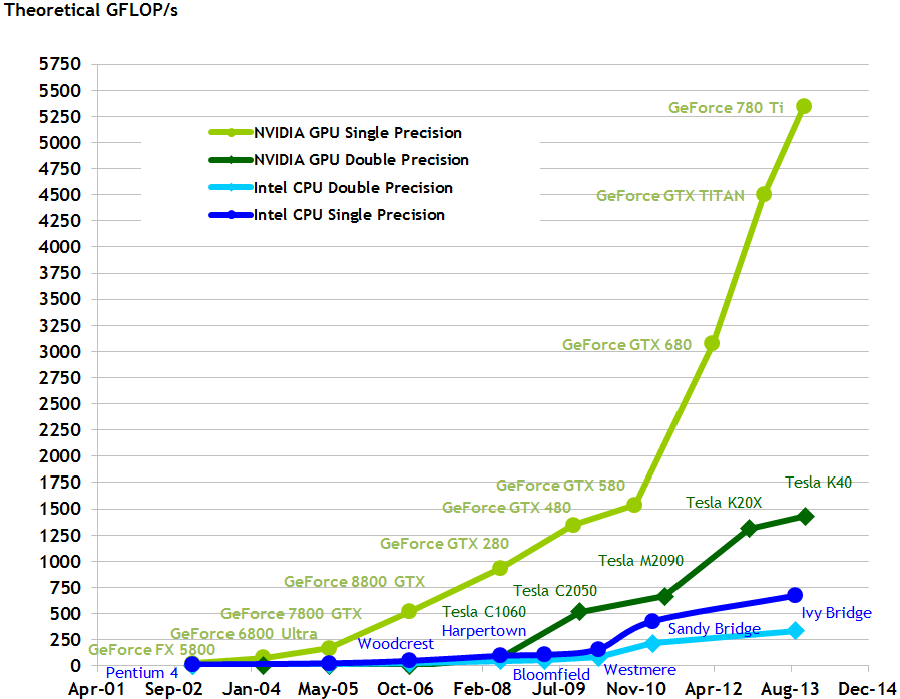
\includegraphics[width=\textwidth]{img/gpu_performance.pdf}
  \caption{Increase in floating-point operations per second for CPUs versus GPUs over time.}
  \label{fig:gpu_performance}
\end{figure}

The huge difference in performance mainly derives from the number of independent compute cores. Even though each individual core of a traditional CPU is very fast they usually only have four, eight or maybe sixteen cores. In contrast to this GPUs can have several hundreds of indepedent compute cores. Each core can simulatenously perform calculations and thus provides the opportunity to yield big performance improvements for high-throughput type computations. This fact also introduced general purpose computing on GPUs to the world of supercomputers. Over time, a growing number of them started supplimenting their compute power with GPUs and some even rely exclusively on GPUs for their computations.

In order to take advantage of these new massively parallel architectures new Application Programming Interfaces (API) had to be developed. The two proposed APIs are OpenCL and CUDA. OpenCL is an open and cross platform standard maintained by the Khronos Group. The same group is also responsible for its graphics focused counterpart OpenGL. OpenCL is not exclusive to GPUs, but instead tries to be a general abstract layer for different parallel architectures. This allows OpenCL code to be run not only on GPUs but also on CPUs and other new hardware like Intels Xeon Phi. CUDA on the other hand is developed by Nvidia exclusively for their line of GPUs.

Choosing between OpenCL and CUDA is the first decision to be made when starting to implement a new project on GPUs. The main advantage of OpenCL is the ability to be able to run on many different devices. All major players in the computing space provide an implentation on top of their platforms. Both Intel and AMD provide the API for their CPU and both AMD and Nvidia have drivers available for their GPUs. However, this advantage can also be a disadvantage as the achievable performance might suffer from the abstraction across all platforms. The OpenCL framework is potentially not optimized for a particular device specific architecture. CUDA on the contrary is in theory highly optimized to achieve the best possible performance on Nvidia's GPUs. In practice the difference can possibly be mitigated by spending the extra time to fine-tune the OpenCL implementation to the hardware's specific needs. Another disadvantage of OpenCL is the potentially outdated and inconsistent driver support for the various devices. This is especially true for Nvidia who seem to have stopped updating OpenCL, still only supporting OpenCL 1.1 which was released back in 2010. Their main focus is on pushing CUDA and updating it to support all the feature in their new GPUs.

For this thesis I chose to go with Nvidia's CUDA framework mainly because of the available hardware both at the workstation computers as well as at the local computing cluster. Additionally this project does not need the cross-platform capability as the main focus is on pure performance in a highly specialized setup and simulation scenario. The application will not be widely distributed and only used for internal purposes.

\section{CUDA}
The CUDA stands for Compute Unified Device Architecture and was introduced by Nvidia in 2006 as a general purpose parallel computing platform. It leverages the highly parallel architecture of modern Nvidia GPUs to solve many different computational problems, which can lead to potentially large performance improvements compared to traditional CPUs.

The CUDA platform allows developers to use a variety of different options to program the GPU. The easiest way is to link to any CUDA-accerlated library and simply using the libraries interfaces from any software environment. For more advanced uses extensions to various programming languages exist like C/C++, Fortran and even managed languages like Java and Python and many more. This allows for easy and fast integration into any software environment the developer is comfortable with. figure~\ref{fig:cuda_overview} illustrated the different components of the overall CUDA platform.

\begin{figure}
  \centering
  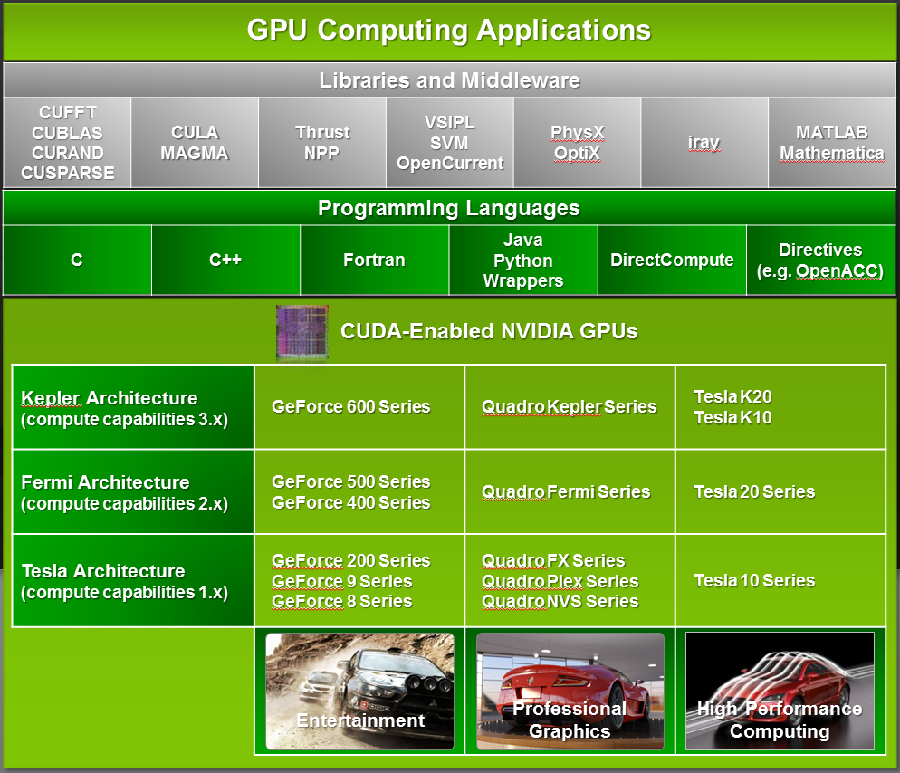
\includegraphics[width=\textwidth]{img/cuda_overview.pdf}
  \caption{Overview of the CUDA platform.}
  \label{fig:cuda_overview}
\end{figure}

The basic building blocks of the CUDA Programming Model from a development perspective are kernels. CUDA kernels are the equivalent of normal C functions. However the major difference is that instead of being executed just once, kernels are executed in parallel by $N$ different threads. These CUDA threads are distributed and run across the available compute cores of the GPU. To illustrate how a very basic kernel call looks, figure \ref{lst:code_vector_addition} shows a code sample for a very simple vector addition.

\paragraph{CUDA Kernels}

\begin{listing}
  \centering
  \begin{minted}[mathescape,
    linenos,
    numbersep=5pt,
    fontsize=\footnotesize,
    frame=lines,
    framesep=2mm]{c}
// Kernel definition
__global__ void VecAdd(float *A, float *B, float *C)
{
  int i = threadIdx.x;
  C[i] = A[i] + B[i];
}

int main()
{
  ...
  // Kernel invocation with N threads
  VecAdd<<<1,N>>>(A,B,C);
  ...
}
  \end{minted}
  \caption{Pseudocode for CUDA vector addition}
  \label{lst:code_vector_addition}
\end{listing}

It is important to remember that each kernel invocation is executed independently and no ordering is guaranteed. It is therefore essential to make sure to avoid any race conditions or shared memory access. There are however, ways to allow for shared memory access which will be briefly touched upon later in the practical implementation of the simulation.

\paragraph{Thread hierarchy}

In order to efficiently distribute the different threads across the compute cores of the GPU, CUDA defines a thread hierachy. As discussed previously a GPU consists of many independent compute cores. On Nvidia GPUs theses cores are referred to as Streaming Multiprocessors (SMs). During execution of the application each SM is tasked with running a distinct set of threads. In CUDA these sets of threads are called thread blocks. Each thread block is then distributed to all the available SMs, which allows for automatic scalability depending on the number of SMs available  as illustrated in figure~\ref{fig:automatic_scaling}.

\begin{figure}
  \centering
  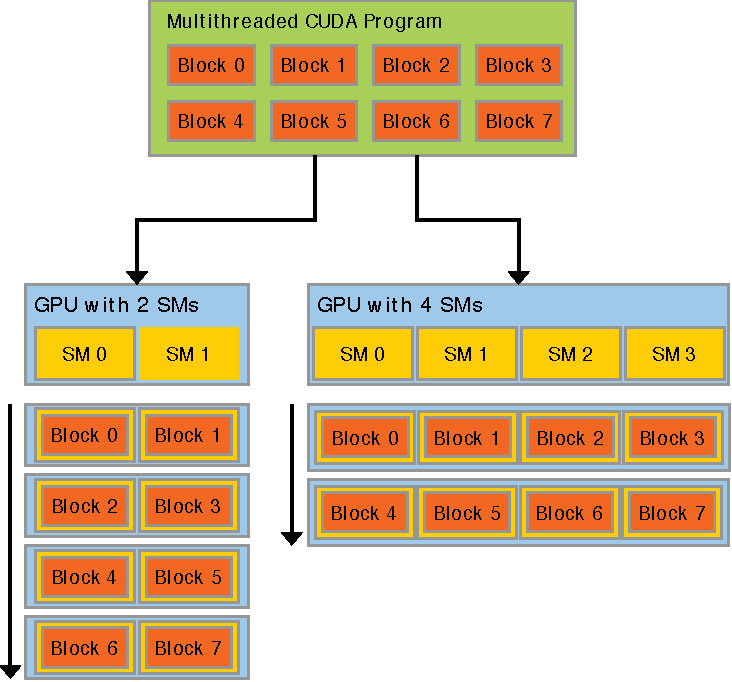
\includegraphics[width=\textwidth]{img/automatic_scaling.pdf}
  \caption{Automatic scaling of blocks across an arbitrary number of Streaming Multiprocessors.}
  \label{fig:automatic_scaling}
\end{figure}

Thus the developer only has to divide the workload into appropriately sized blocks of threads and invoke the kernel. How to choose the optimal size of a block to maximize the performance is not an easy question to answer and is highly dependent on the particular task and implementation. In practice the size is often chosen by running benchmarks with various different sizes to determine the sweet spot.

In order to make programming and modeling of real world problems easier CUDA blocks can be addressed using either a one-dimensional, two-dimensional, or three-dimensional thread index. For example in the case of a matrix calculation it is more natural to think about parallelizing each element given by the row and column index instead of a single one-dimensional index. This is illustrated in the code simple in listing~\ref{lst:code_matrix_addition}

\begin{listing}
  \centering
  \begin{minted}[mathescape,
    linenos,
    numbersep=5pt,
    fontsize=\footnotesize,
    frame=lines,
    framesep=2mm]{c}
// Kernel definition
__global__ void MatAdd(float A[N][N], float B[N][N], float C[N][N])
{
  int i = threadIdx.x;
  int j = threadIdx.y;
  C[i][j] = A[i][j] + B[i][j];
}

int main()
{
  ...
  // Kernel invocation with one block of N * N * 1 threads
  int numBlocks = 1;
  dim3 threadsPerBlock(N, N);
  MatAdd<<<numBlocks, threadsPerBlock>>>(A,B,C);
  ...
}
  \end{minted}
  \caption{Pseudocode for CUDA matrix addition, illustrating 2D thread blocks}
  \label{lst:code_matrix_addition}
\end{listing}

Finally because the resources of each Streaming Multiprocessor are limited there exists a upper bound of how many threads a block can contain. Currently this maximum number of threads is $1024$. This means that the maximum size of matrices possible to be added in the code sample in listing~\ref{lst:code_matrix_addition} is $32\times32$. To solve this problem CUDA introduces another layer above blocks called a grid. A grid organizes thread blocks again into either one, two, or three dimensions. The number of thread blocks in a grid is unlimited and thus solely dependent on the size of the workload. Listing~\ref{fig:grid_blocks} shows an example configuration of a 2D grid with 2D blocks.

\begin{figure}
  \centering
  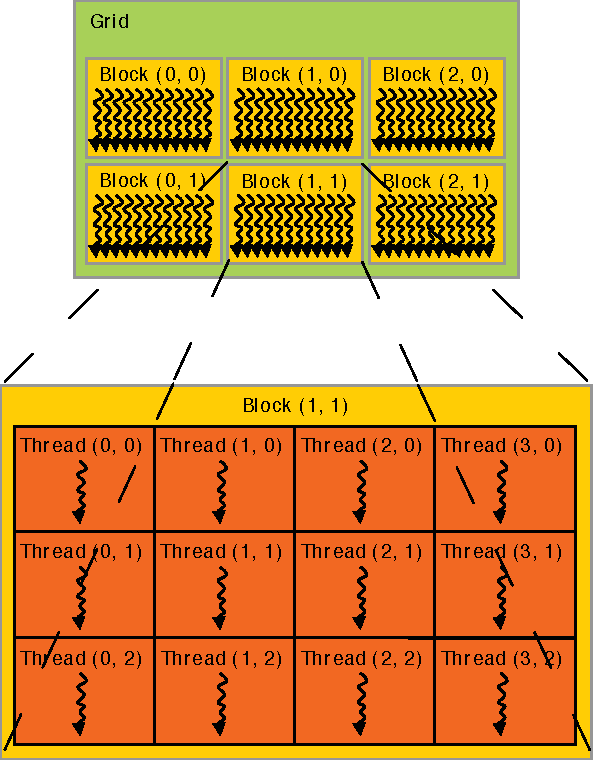
\includegraphics[width=0.6\textwidth]{img/grid_blocks.pdf}
  \caption{Overview of the CUDA platform.}
  \label{fig:grid_blocks}
\end{figure}

\paragraph{Memory hierarchy}

In addition to the Thread hierarchy...

\begin{itemize}
\item 4 Layers, Global, Local, Private
\item Global shared across all SM
\item Local shared across thread block
\item Private per thread
\item Latency VERY different between layers
\item Avoid global memory access
\item Or hide with compute heavy, as is the case with assemble system step (ala will be used later)
\end{itemize}

\section{Implementation}
The rigid fiber simulation developed as part of this thesis is only loosely based on the original serial Fortran implementation. This was done to ensure a clean starting point and avoid difficulties in adapting the existing code for parallel execution as it was never intended to be run across multiple cores. This also provided the opportunity to learn from the shortcomings of the old code to not only parallelize it but also improve the efficiency in general.

The development was done exclusively on a Linux workstation running Ubuntu as this will also be the exact same runtime environment used in the later experimental usage of the resulting application. The build system for compiling and linking the final application was CMake. It was chosen because it is widely used open-source and cross-platform build system, which allowing for easy integration of the various required libraries in a well documented and straightforward manner.

Under the hood the build system uses Nvidia's CUDA platform tools and to compile the code. For this Nvidia includes \emph{nvcc}, an LLVM-based CUDA compiler capable of compiling C/C++ code combined with CUDA specific extensions. In addition to the CUDA libraries the application also requires support libraries for the different linear solvers. The two main libraries are \emph{MAGMA} for the direct solver and \emph{ViennaCL} for the iterative solvers. Both will be introduced briefly now.

\paragraph{MAGMA / CuBLAS / OpenBLAS}
The MAGMA project provides the implementation for the direct solver used during this thesis. This dense linear algebra library provides features similar to standard LAPACK functions but for multicore architectures. It also provides features to support hybrid algorithms across multiple different archictures, however these features where not explored in this thesis. Instead the focus was on a high performant single GPU implementation of a direct linear system solver.

MAGMA provides the interfaces for various high-level languages, however the underlying math functions utilize the platform specific implementations of the BLAS levels. For CUDA this is provided directly by Nvidia in the form of the CuBLAS libraries. Additionally MAGMA tries to be as fast as possible which sometimes means integrating CPU based algorithm where it makes sense. Thus a CPU based BLAS implementation is also needed. For this I chose the OpenBLAS library which is the most up to date and high performant library available outside the very expensive Intel MKL library. OpenBLAS takes full advantage of multicore systems using pthreads and is also used for the comparison of Fortran CPU implementation against the CUDA GPU implementation

\paragraph{ViennaCL}
ViennaCL is an open-source linear algebra library developed at the Universiy of Vienna. The library provides an abstraction layer across many different parallization methods in order to provide consistent and easy to use support for BLAS level 1-3 and iterative solvers. This unique feature allows the developer to easily switch between different backends for parallelization. Currentely the library support OpenMP, OpenCL and most importantanly for this thesis CUDA.

While mostly focussed on sparse matrices for the implemented iterative solvers, ViennaCL also support solving dense matrices using a variety of different iterative solvers. As the rigid fiber simulation exclusive relies on dense matrices this makes it an ideal candidate for benchmarking. For this thesis both the BiCGStab as well as the GMRES iterative solvers where used and tested.

In order to faciliate easier usage of application both during development and later real-world usage a Python wrapper script is also available. The script completely automates the building process and dynamically customizes the application code to support three different modes of operation. The first is a simple \emph{run} mode which simply takes the supplied parameters and executes the simulation. The second mode is \emph{validate}, it allows for a fully automated way to test and validate different algorithm variantions against a known correct simulation run. This includes automatically computing the error as well as the error location in the matrix allowing for easier debugging of changes. The last mode is \emph{benchmark} which run the supplied parameters through a series of iterations collecting and aggregating timings for each simulation step as well as the total time.

Unified interface for OpenMP and CUDA -> OpenMP only introduced later?!? -> Is that really important any way?

\subsection{Kernels}
The overall parallel algorithm is very similar to the serial version, however each simulation step is seperated into different kernels. Each kernel is invocate in a serial manner, this means CUDA guarantess that all data modified in a kernel is available before the next kernel is executed. These kernels are than distributed across the GPU. All calculations are done using single precision floating point numbers, as Nvidia limits high performance double precision computation to their server class GPUs. The CUDA pseudocode for algorithm is illustrated in listing~\ref{lst:pseudo_parallel_algorithm}.

\begin{listing}
  \centering
  \begin{minted}[mathescape,
    linenos,
    numbersep=5pt,
    fontsize=\footnotesize,
    frame=lines,
    framesep=2mm]{c}
int main()
{
  // Parsing algorithm parameters and initial fiber positions
  readParameters();
  readSetup();
  allocateGPUMemory();
  ...

  for (int step = 0; step < max_timestep; step++)
  {
    AssembleSystem<<<numBlocks, threadsPerBlock>>>(...);
    SolveSystem<<<numBlocks, threadsPerBlock>>>(...);
    UpdateVelocities<<<numBlocks, threadsPerBlock>>>(...);
    UpdateFibers<<<numBlocks, threadsPerBlock>>>(...);
  }
  ...
}
  \end{minted}
  \caption{Pseudocode for parallel algorithm on the host.}
  \label{lst:pseudo_parallel_algorithm}
\end{listing}

The application requires two general configuration files as an input. The first file is referred to as the parameters file which contains the different configuration variables and constant used throughout the algorithm. These include for example the number and size of the timesteps as well as the number of force expansion terms and number of quadrature points. Additionally this file is also used to

Each of the parallized substeps are now discussed in more detail. I will discuss the purpose of each kernel as well as the required input and outputs.

\paragraph{Assemble System}

\begin{listing}
  \centering
  \begin{minted}[mathescape,
    linenos,
    numbersep=5pt,
    fontsize=\footnotesize,
    frame=lines,
    framesep=2mm]{c}
__global__ void AssembleSystem1D(
  in float *positions,
  in float *orientations,
  out float *a_matrix,
  out float *b_vector)
{
  const int i = blockIdx.x * blockDim.x + threadIdx.x;

  if (i >= NUMBER_OF_FIBERS) return;

  for (int j = 0; j < NUMBER_OF_FIBERS ++j)
  {
    for (int force_index_j = 0; force_index_j < NUMBER_OF_TERMS_IN_FORCE_EXPANSION; ++force_index_j)
    {
      computeInnerIntegral(...);

      for (int force_index_i = 0; force_index_i < NUMBER_OF_TERMS_IN_FORCE_EXPANSION; ++force_index_i)
      {
        // Only 1D thread block
        // Each thread updates unique memory locations, thus
        // no need for atomics
        setMatrix(...)
        setVector(...)
      }
    }
  }
}
  \end{minted}
  \caption{Pseudocode for the assemble system step with a 1D thread block.}
  \label{lst:pseudo_assemble_system}
\end{listing}

The \emph{Assemble System} kernel is the most important step of the algorithm. Its goal is to build the matrix and vector in memory for the linear system of equations in the form of $A*x = b$. Listing~\ref{lst:pseudo_assemble_system} shows the pseudocode for the one-dimensional implementation of the assemble system step. This means the code is parallized for each fiber and each thread calculates the contributions to this fiber form all other fibers. Looking at the matrix each thread is thus responsible for $3*M$ rows of the matrix.

The kernel requires two inputs, the current position of the each fibers and its orientation. Using these combined with the equations outlined in chapter~\ref{cha:theoretical_foundation} and chapter~\ref{serial_implementation} the matrix and vector elements are computed and used in the next step to solve the linear system they define.

\paragraph{Solve System}
As this thesis does not aim to implement generic linear solvers, this step is treated as a black box. During the previous \emph{Assemble System} kernel two arrays containing the matrix and right hand side of the linear system have been computed. These two arrays are now passed to the respective function of the library containing the linear solver. This is the MAGMA library in case of the direct solver and the ViennaCL library in case of the two tested iterative solvers BiCGStab and GMRES. Both libraries are able to directly use the already allocated memory regions and no additional allocations have to be performed. In order to conserve memory space the resulting solution vector is stored in the same memory location as the $b$-vector and is passed on to the the subsequent steps.

\paragraph{Update Velocities}

\begin{listing}
  \centering
  \begin{minted}[mathescape,
    linenos,
    numbersep=5pt,
    fontsize=\footnotesize,
    frame=lines,
    framesep=2mm]{c}
__global__ void UpdateVelocities2D(...)
{
  const int i = blockIdx.x * blockDim.x + threadIdx.x;
  const int j = blockIdx.y * blockDim.y + threadIdx.y;

  if (i >= NUMBER_OF_FIBERS) return;
  if (j >= NUMBER_OF_FIBERS) return;
  if (i==j) return;

  for (int quadrature_index_i = 0; quadrature_index_i < TOTAL_NUMBER_OF_QUADRATURE_POINTS; ++quadrature_index_i)
  {
    for (int quadrature_index_j = 0; quadrature_index_j < TOTAL_NUMBER_OF_QUADRATURE_POINTS; ++quadrature_index_j)
    {
      force = computeForce(coefficents, ...)
      computeDeltaVelocities(force)
    }
  }

  // 2D thread block
  // Each thread responsible for an interaction pair, thus
  // result is written to the same memory location
  // Using atomics to avoid conflicts
  atomicAdd(&(translational_velocities[i].x), delta_translational_velocity.x);
  atomicAdd(&(translational_velocities[i].y), delta_translational_velocity.y);
  atomicAdd(&(translational_velocities[i].z), delta_translational_velocity.z);

  atomicAdd(&(rotational_velocities[i].x), delta_rotational_velocity.x);
  atomicAdd(&(rotational_velocities[i].y), delta_rotational_velocity.y);
  atomicAdd(&(rotational_velocities[i].z), delta_rotational_velocity.z);
}
  \end{minted}
  \caption{Pseudocode for the updating velocities simulation step.}
  \label{lst:pseudo_update_velocities}
\end{listing}

After solving the linear system the solution coefficents are used to update the velocities of the fibers. The \emph{Update Velocities} kernel accumulates the excerted forces for all fibers and updates both the translational as well as the rotational velocities simultaneously. In this particular instance the 2D thread block version of the kernel is illustrated in listing~\ref{lst:pseudo_update_velocities}. This means each individual kernel invocation is responsible for a single pair of fiber interaction. Under the normal assumption that kernel invocations are not allowed to write to the same memory location this would result in undefined behaviour and incorret results for the velocities.

Fortunately CUDA provides a mechanism to circumvent this issue. By using so called atomic function CUDA streamlines and serializes the memory access. Thus the atomicAdd function accumulates different velocity contributions to a fiber from all the other fibers. This ensures that each update to the memory location is handled in a serial manner, guararenteeing the correct value in memory for each. Of course this implies a potential performance degradation, however newer GPUs with new CUDA version have been very well optimized to only have a minimal negligible impact. Benchmarking for the fibers simulation show that using a 2D thread block and the associated performance increases for outweight the potential performance hit of using atomics.

\paragraph{Update Fibers}

\begin{listing}
  \centering
  \begin{minted}[mathescape,
    linenos,
    numbersep=5pt,
    fontsize=\footnotesize,
    frame=lines,
    framesep=2mm]{c}
__global__ void UpdateFibers()
{
  int i = blockIdx.x * blockDim.x + threadIdx.x;

  if (i >= NUMBER_OF_FIBERS) return;

  next_positions[i] = 4/3 * current_positions[i]
    - 1/3 * previous_positions[i]
    + 2/3 * TIMESTEP
      * (2 * current_translational_velocities[i] - previous_translational_velocities[i]))

  next_orientations[i] = 4/3 * current_orientations[i]
    - 1/3 * previous_orientations[i]
    + 2/3 * TIMESTEP
      * (2 * current_rotational_velocities[i] - current_rotational_velocities[i]))

  normalize(next_orientations)
}
  \end{minted}
  \caption{Pseudocode for the updating fibers simulation step.}
  \label{lst:pseudo_update_fibers}
\end{listing}

The final simulation step takes care of advancing the position and orientation of the fibers in time. The pseudecode in listing~\ref{lst:pseudo_update_fibers} implements the second-order multi-step method introduced in section~\ref{sec:time_stepping}. As seen later in the results in chapter~\ref{cha:results} this required time for this kernel is minuscule compared to the other steps. The kernel only scales linearly and additional has a perfectly aligned memory access resulting in close to optimal usage of the GPU hardware.

\subsection{Optimizations}

During the developement of the parallel GPU simulation great care was taken to continously optimize the code both on an algorithmic level as well as on an implementation level. Numerous small code-level optimizations have been performed based on the original serial code like precomputing as much data as possible, avoiding variable allocations or unnecessary copy operations in performance critical sections of the code.

Additionally more advanced optimization like rearranging calculations inside loops to avoid executing redundant calculations and consolidating multiple loops into one. Finally techniques such as loop unrolling and faster math functions where also tested and included.

Throughout the optimization phase the benchmark suite was run after each step. This ensures that optimizations where only included if they had a measureably impact on the overall performance of the simulation. Moreover in this way potential performance regressions could be identified early and be avoided.

Many optimizations performed during this process are applicable to both the CPU and GPU and show performance improvements for both. However some optimizations or algorithm variantions have a either a different effect or are uniquely suited and related to the GPU hardware. For this thesis we will look into three general different optimizations in more detail. The performance results for each will then later be discussed in chapter~\ref{cha:results}

\subsubsection{Numeric vs. Analytic Integration}
The first optimization was already part of the original serial implementation as described in section~\ref{sec:}. In the original paper \cite{} the authors observed that the analytical integration of the inner integral yielded a performance increase compared to the numerical integration. On paper an analytical integration should also not only be preferred by being faster but more importantly also being more accurate.

However for numerical precision reasons the actual implementation of the analytical integration can't achieve this theoretical level of accurary. The implementation is dependent on design variable ensuring numerically stable results for very close fibers. The computation of the inner integral lies at the heart of the algorithm and is a very performance critical section of the implementation. So in order to explore the performance implications of both approaches on GPU especially compared against CPU is of great interest.

\subsubsection{Shared Memory}

As the described in section~\ref{} CUDA code is subject to a highly specilizated memory hierarchy. Whereas traditional CPUs only have small caches and a large main memory pool, CUDA introduces the concept of a shared local memory space. This access time to this local memory is orders of magnitudes faster compared to accessing the global GPU memory. Additionally local memory can be shared among a CUDA thread block and potentially save time by avoiding to constantly access the slow global memory.

In order to test this shared memory was implemented and tested with the \emph{Assemble System} step, the most performance critical kernel written for the fiber simulation. To understand the idea imagine the 2D thread block implementation of the kernel. Each thread block is responsible for many pairs of fiber interactions, e.g. fibers $[1,8]$ each interacting with fibers $[9,16]$. In total these are $8 \times 8 = 64$ interactions. Each kernel invocation is responsible for one pair and has to load the position and orientation for the two interacting fibers. However on closer inspection it is obvious that one does not need to load each fiber every time. As soon as fiber $1$ has been loaded into shared memory in can be reused for all the interactions with fibers $9$ throught $16$ avoiding the unnecessary and slow access to global memory.

How this affects performance however is not always easy to tell, as various factors can influence the result. If the loaded data is small enough the various memory caches can hide to increased costs of accessing global memory. Also while the first threads in a thread block load the data from global to shared memory all other threads in this thread block have to wait for their data to become available. This is especially true if the overall kernel has to execute many calculations and the required time for computations effectively hides the memory loading time as CUDA is able to simply switch to the next thread block and continue executing it. In this case the performance penatly only occurs at the very beginning and end, and has only a negible impact on the overall performance.

However in general efficient exploitation of shared memory can be a huge advantage for parallel GPU implementations. This is especially true because CPUs don't have an equivalent fast and comparatively large memory space. It is therefore an interesting optimization to explore and benchmark.

\subsubsection{Thread Block Dimension}

There are many different factors that determine the performance of a particular GPU algorithm. This is especially true with regards to optimally taking advantage of the specific underlying GPU architecture which change even between different models of graphics cards. How to best utilize the hardware depends on specific memory access patterns, avoiding too much register usage and choosing optimal settings for the thread block size. Each graphics cards can have a different number of streaming multiprocessors with only limited resources and taking advantage of this can result in performance increases.

For this thesis we looked at the Thread Block dimension in particular and how choosing a different approach to parallizing affects the performance, again with a focus on the \emph{Assemble System} step as the most performance critical step. However the results were then also transferred to the \emph{Update Velocities} step.

The most straight forward approach is to simply parallize the algorithm with regards to a single fiber. This means each kernel invocation is responsible for calculating all the interactions for this fibers with all other fibers. In this way a single kernel is responsible for multiple rows of the resulting linear system matrix. Additionally this approach does not have any memory access conflict as each kernel only writes to the memory location belong to its unique fiber. The potential disadvantage for a one-dimensioanal thread block however is that the resulting code can be more resource intensive for each single kernel and potentially hinder to performance on each multiprocessor.

For a two-dimensional thread block each kernel invocation is responible for a pair of fibers interacting. While this decrease the needed resources it also required atomics which can potential slow down the execution. Three-dimensional thread blocks are the maximum allowed dimensions for a CUDA thread block. They are the a further extension of the two-dimensional thread block, as now each kernel invocation is responsible for not the complete interaction but only the interaction resulting from a specific point from the force expansion. This results in even more potential memory conflicts and also increases the total number of thread blocks which have to be distributed.

How exactly each decision for the thread-block dimension affects performance is not clear. Only trial-and-error benchmarking combined with metrics from CUDA can find the optimal setting for the specific algorithm.

\section{OpenMP}

The goal of this thesis is to implement a high performant rigid fiber simulation on the GPU using CUDA. However in order to better understand to what degree this goal was achieved it would be nice to have comparison. The original serial implementation is not an ideal candidate has it does differ in a number of ways. First of all its purely serial not even taking advantage of todays multicore CPUs. Furthermore it was implemented in double precision and first practical restrictions on consumer CUDA GPUs are only really well suited for single precision, for this reason the CUDA is only single precision. Finally the primary focus of the original Fortran implementation was a correctly implemented algorithm and not performance.

For these reasons and in order to have a fairer comparsion of the performance differences of the GPU and CPU implementation a completely new and rewritten parallel CPU simulation was also implemented. For the parallization the OpenMP library was chosen.

- What is OpenMP

After having implemented a parallel algorithm for the GPU the conversion to the OpenMP-based CPU implementation was relatively straightforward. Almost all optimizations for the GPU implementation where also applied to the new CPU code. In order to parallize the BLAS functions required for the linear solver the already included OpenBLAS library was chosen. OpenBLAS is both open-source and highly optimized and automatically parallizes BLAS functions using pthreads across all available CPU cores. In contrast to the GPU implementation is only parallized in one-dimension, so each core calculates the iteractions for one fiber with all other fibers, or put differently all matrix rows belong to one fiber. As the underlying number of independently threads is much lower on CPUs, different parallization dimension didn't have an impact during testing.

The end results of the practical implementation for this thesis is a highly optimized CUDA implementation for Nvidia GPUs and additionally a parallized and optimized Fortran OpenMP implementation for CPUs. The next chapter will now look at a number of performance metrics and compare them between the GPU and CPU.

\chapter{Results}
The last chapter introduced the parallel implementation of the numerical simulation. It introduced the concept of general purpose computing on modern GPUs as well as giving a practical overview of the implementation of the algorithm using nVidia CUDA framework and possible optimiziations to take advantage of the unique properties of the GPU architecture.

Using all the available implementations of the algorithm this chapter will showcase a multitude of different result and benchmarks performed. This is done to illustrate the achieved performance increases on the GPU over the original serial CPU implementation and the parallel OpenMP implementation.

\section{Examples}

Before examining the different performance metrics and optimizations we will first look at a couple of examples to better illustrate the rigid fiber simulation. The first example shows the numerical precision of the final single precision simulation compared against both the original serial double precision and at the expected physical results. The second example illustrates a real world example which illustrates an interesting phyiscal phenomen. Both a run with the fastest CUDA algorithm implemented in the thesis.

\subsection{Numerical precision}
\subsection{Sphere simulation}

\begin{figure}
  \centering
  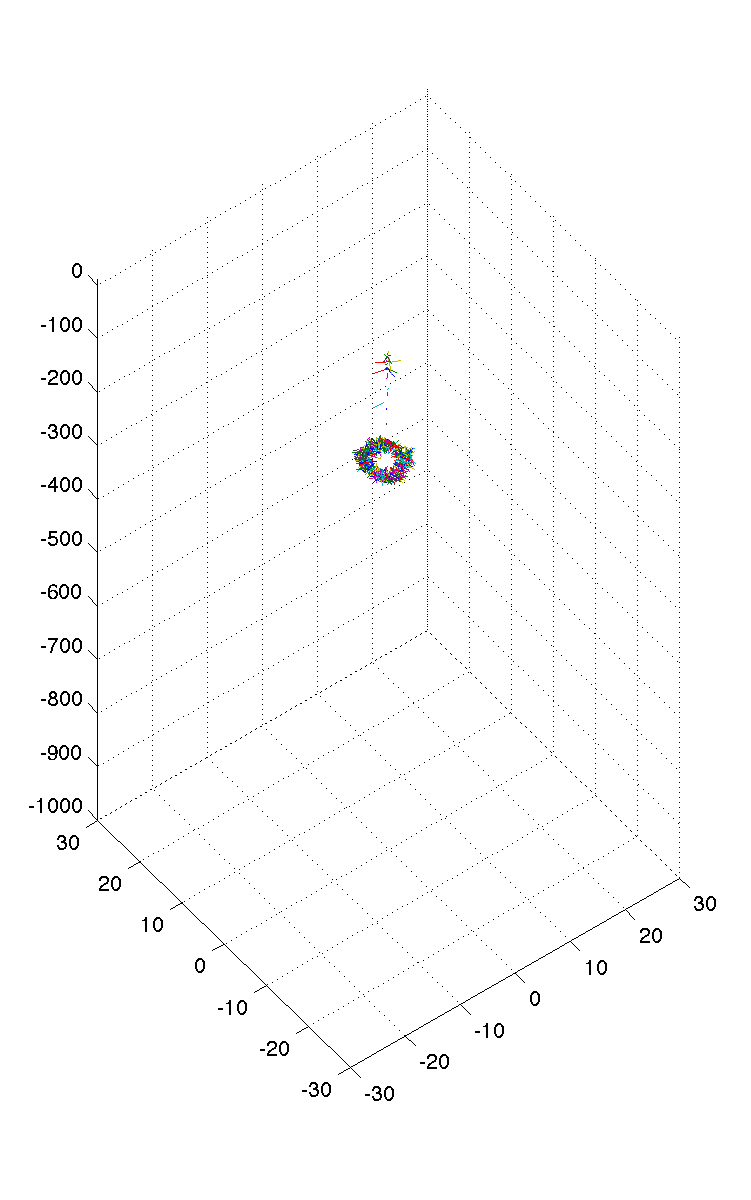
\includegraphics[width=0.2\textwidth]{img/sphere_00100.png}
  \caption{t=100}
  \label{fig:sphere_simulation}
\end{figure}

\section{Methodology}

The methodology used for the benchmark suite is the same for all presented benchmarks. This ensure comparable results and fairest comparison possible.

\subsection{Hardware}

All benchmarks were run on a the same workstation with specifications listed in table XX.


\begin{center}
\begin{tabulary}{0.7\textwidth}{LL}
  \toprule
  \multicolumn{2}{c}{Workstation} \\
  \midrule
  Processor & Intel Core i7 4770 \\
  Graphics & Nvidia GTX 970 4GB \\
  RAM & 16GB DDR3 \\
  Operating System & Ubuntu Linux 12.04 LTS \\
  CUDA Driver & CUDA 6.5.xxxx \\
  \bottomrule
  \label{tab:workstation}
\end{tabulary}
\end{center}

\subsection{Benchmark scheme}

The main goal of the benchmark system was to generate statistical significant and reproducable performance numbers. To ensure this all benchmarks for both the GPU and the CPU were run using the exact same scheme. In order to obtaining the timings the builtin CUDA timing events were used for each individual kernel. For Fortran the \emph{SYSTEM\_CLOCK} function was used respectively.

For all different benchmarks timings were obtained for a different number of fibers starting from $100$ up to $2000$ in $100$ increments. For each seperate number of fibers a number of iterations are run to obtain the average over multiple runs. For each iteration a completely new and random initial fiber configuration is generated with the current number of fibers. In order to exclude illegal configurations where fibers overlap and intersect an additional correction pass is done over the fibers to ensure a minimal and average distance between all fibers. For the configrations in this thesis the minimal distance was always set to $0.2$ and the average to $0.4$ respectively.

Using this semi-random generation the rigid fiber simulation is run for exactly $10$ timesteps. To avoid remaining outliers in the configuration causing potentially large variation in the timings especially for iterative solvers the first timestep is excluded from the timing and instead used as a simple warmup step for the simulation. So the final average time for each run is taken from the last $9$ timesteps.

In order to ensure a stasticial sgnificant result the number of iterations is not fixed, instead it is determined dynamically based on the relative standard error of the already collected timing for the particular number of fibers. Beginning with a minimum of number iterations the relative standard error of the total times is calculated. If the relative standard error of the dataset is larger than a specificed threshold the number of iterations is doubled and run again. The benchmark suite uses a minimum of $4$ iterations to obtain the initial timings if the relative standard error is not below a threshold of $20\%$ an additional $4$ iterations are run to bring the total to $8$. This process repeats until the threshold is satisfied and more reliable benchmark timings have been obtained. This algorithm is illustrated using pseudocode in listing~\ref{lst:pseudo_benchmark}.

\begin{listing}
  \centering
  \begin{minted}[mathescape,
    linenos,
    numbersep=5pt,
    fontsize=\footnotesize,
    frame=lines,
    framesep=2mm]{c}
for(int N = 100; N <= 2000; N += 100)
{
  int iterations = 4;
  while (iterations <= MAX_ITER)
  {
    for(int i = 0; i < iterations; ++i)
    {
      generateRandomInitialFiberConfiguration();
      run(10); // execute 10 timesteps
      collectTimings();
    }

    rse = calculateRelativeStandardError();

    if (rse <= 0.2)
    {
      break;
    }

    iterations *= 2
  }

  reportTimings();
}
  \end{minted}
  \caption{Pseudocode for benchmark scheme.}
  \label{lst:pseudo_benchmark}
\end{listing}

\section{Optimizations}

We now look at the performance results for the different optimizations previously outlined in section~\ref{sec:implementation_optimization}. Where applicable the results will be compared between the OpenMP and CUDA version of the algorithm.

\subsection{Numeric vs. Analytic Integration}

The first benchmark tests the performance of the two different approaches to compute the inner integral. It can be solved either numerically or analytically. Figure~\ref{fig:openmp_num_vs_anal} illustrates the performance timings for the \emph{Assemble System} step of the parallel OpenMP version. Inline with the observations made by the authors of the original serial implementation the parallel version of the analytic integration is always faster than the numeric integration.

\begin{figure}
  \centering
  \begin{tikzpicture}
    \setmathfont{FiraSans-Book.otf}
    \begin{axis}[
      title=OpenMP Numeric vs. Analytic Integration,
      xlabel={number of fibers},
      ylabel={simulation time (sec)},
      ymin=0,ymax=55,
      xmin=0,xmax=2000,
      unbounded coords=discard,
      ]
      \addplot[color=set11,mark=*,mark options={fill=white}, very thick] table[x=X,y=ASSEMBLE_SYSTEM] {benchmarks/openmp_direct_numerical.csv};
      \addplot[color=set12,mark=*,mark options={fill=white}, very thick] table[x=X,y=ASSEMBLE_SYSTEM] {benchmarks/openmp_direct_analytical.csv};

      \legend{Numerical, Analytical}
    \end{axis}
    \setmathfont{XITS Math}
  \end{tikzpicture}
  \caption{Benchmark of assemble system step for integration of inner integral.}
  \label{fig:openmp_num_vs_anal}
\end{figure}

However the picture is more interesting when we look at the same graph for the CUDA implementation in figure~\ref{fig:cuda_num_vs_anal}. Here the results are reversed. The numeric integration out performs the analytical integration by an larger margin increasing with the number of fibers.

\begin{figure}
  \centering
  \begin{tikzpicture}
    \setmathfont{FiraSans-Book.otf}
    \begin{axis}[
      title=CUDA Numeric vs Analytic Integration,
      xlabel={number of fibers},
      ylabel={simulation time (sec)},
      ymin=0,ymax=5.5,
      xmin=0,xmax=2000,
      unbounded coords=discard,
      ]
      \addplot[color=set11,mark=*,mark options={fill=white}, very thick] table[x=X,y=assemble_system] {benchmarks/cuda_bicgstab_numerical_2D.csv};
      \addplot[color=set12,mark=*,mark options={fill=white}, very thick] table[x=X,y=assemble_system] {benchmarks/cuda_bicgstab_analytical_2D.csv};

      \legend{Numerical, Analytical}
    \end{axis}
    \setmathfont{XITS Math}
  \end{tikzpicture}
  \caption{Benchmark of assemble system step for integration of inner integral.}
  \label{fig:cuda_num_vs_anal}
\end{figure}

This reason for this result lies in the way work is scheduled and executing on the GPU. All code inside a thread block (more precisely a warp) is always executed in lockstep. This means each line of code is executed for each thread in parallel. However if the code encounteres a branch in the execution path like a simple \emph{if} statement the threads diverge. First all threads for which the condition hold true execute while the other threads have to wait. Only after that can the threads with the false condition execute while the other threads are not used. Finally after all divergent paths have been executed the code continous in lockstep. This issue is referred to as Branch Divergence and should be avoided as much as possible when writing parallel GPU Code.

To confirm that Branch Divergence is the reason for the slow down of the analytic integration on the GPU we look at the metrics of the CUDA profiler \emph{nvprof}. The metric \emph{Warp Execution Efficency} shows the ratio of the average active threads per warp to the maximum number of threads per warp. The metrics for both the numerical and analytical integration of the Spherical fiber setup used in in section~\ref{sec:example_sphere} can be seen in table~\ref{tab:branch_divergence}.

\begin{center}
  \begin{tabulary}{0.7\textwidth}{LR}
    \toprule
    Algorithm & warp\_execution\_efficiency \\
    \midrule
    Numerical & $99.01\%$ \\
    Analytical & $53.79\%$ \\
    \bottomrule
    \label{tab:branch_divergence}
  \end{tabulary}
\end{center}

On one hand the numerical integration is almost $100\%$ efficient, meaning all warps execute in complete lockstep. The analytical integration on the other hand is only $50\%$ efficient, meaning that most of time only half of threads actually perform work while the other half is just waiting. This results in the observered performance difference. Closer inspection of the source code reveal that the design constant and the resulting branching as described in section~\ref{sec:analytical_integration} is responsible for the divergence. The constant determines a if a different computation is performed in case fibers are very close together. Unfortunately in order to ensure numeric stability this workaround is unavoidable.

\subsection{Shared Memory}

- No effect of the performance
- Assemble System is not Compute Bound not Memory Bound. The transfer times are dwarfed by the compute time

\subsection{Thread Block Dimension}

The next optimization looked at was the Thread Block Dimension on the GPU. Choosing the best option is a trade-off between the resources used overhead caused by an increased amout of memory writes to the same location and thus the need for potential slow atomics.

\begin{figure}
  \centering
  \begin{tikzpicture}
    \setmathfont{FiraSans-Book.otf}
    \begin{axis}[
      title=CUDA Thread Block Dimension,
      xlabel={number of fibers},
      ylabel={simulation time (sec)},
      ymin=0,ymax=1.4,
      xmin=0,xmax=2000,
      unbounded coords=discard,
      ]
      \addplot[color=set11,mark=*,mark options={fill=white}, very thick] table[x=X,y=assemble_system] {benchmarks/cuda_magma_numerical_1D.csv};
      \addplot[color=set12,mark=*,mark options={fill=white}, very thick] table[x=X,y=assemble_system] {benchmarks/cuda_magma_numerical_2D.csv};
      \addplot[color=set13,mark=*,mark options={fill=white}, very thick] table[x=X,y=assemble_system] {benchmarks/cuda_magma_numerical_3D.csv};

    \legend{1D, 2D, 3D}
    \end{axis}
    \setmathfont{XITS Math}
  \end{tikzpicture}
  \caption{Benchmark of assemble system step for different thread block dimensions.}
  \label{fig:bench_cuda_thread_blocks}
\end{figure}

The results in figure~\ref{fig:bench_cuda_thread_blocks} indicate that the best option for this particular GPU is a two-dimensional thread block. Using a three-dimensional thread block is always slower and has a worse scaling factor. Using the \emph{Atomic Transactions} from \emph{nvprof} shows the total number of atomic transationcs that had to be performed. As can be seen in table~\ref{tab:atomic_transationcs} the required atomic transactions are almost two times larger in the 3D case for the Sphere example from section~\ref{sec:example_sphere}.

\begin{center}
  \begin{tabulary}{0.7\textwidth}{LR}
    \toprule
    Algorithm & atomic\_transactions \\
    \midrule
    2D & $1269325$ \\
    3D & $2350670$ \\
    \bottomrule
    \label{tab:atomic_transactions}
  \end{tabulary}
\end{center}

The one-dimensional approach is also slower than either two-dimensional or three-dimensional. However it appears to scale linearly whereas the other two scale exponentially. It can already be observed that 1D becomes faster than 3D for close to $2000$ fibers. Unfortunately the hardware of the workstation does not have enough memory to simulate more fibers. So for this particular hardware setup two-dimensional thread blocks are the fastest option.

\section{Linear Solvers}

Next we compare the performance for different linear solvers. We explored two different types of solver. The first type is a direct solver of the linear equations which is both implemented for OpenMP as well as the CUDA implementation. The second type are iterative solvers. Unfortunately we can't take advantage of the main advantage of iterative solvers to efficiently solve sparse matrices as the system for the rigid fiber simulation is a dense matrix. The time required for solving the linear system is an increasingly large part of the overall runtime. It is therefore very important to find the optimal solver for this particular solver to arrive at the best performing algorithm overall.

On the CPU side we used the direct solver provided by the OpenBLAS library, which is fully parallized. For GMRES we used the single precision Fortran implmentation from Frayssé et al. which takes extensive advantage of the underyling BLAS functions parallized by OpenBLAS. The original paper quotes that they choose GMRES because it was faster than a direct solver for their tests. The benchmark results for this thesis are illustrated in figure~\ref{fig:bench_openmp_solvers}.

\begin{figure}
  \centering
  \begin{tikzpicture}
    \setmathfont{FiraSans-Book.otf}
    \begin{axis}[
      title=OpenMP Linear Solver,
      xlabel={number of fibers},
      ylabel={simulation time (sec)},
      ymin=0,ymax=180,
      xmin=0,xmax=2000,
      unbounded coords=discard,
      ]
      \addplot[color=set11,mark=*,mark options={fill=white}, very thick] table[x=X,y=SOLVE_SYSTEM] {benchmarks/openmp_direct_numerical.csv};
      \addplot[color=set12,mark=*,mark options={fill=white}, very thick] table[x=X,y=SOLVE_SYSTEM] {benchmarks/openmp_gmres_numerical.csv};

      \legend{Direct Solver, GMRES}
    \end{axis}
    \setmathfont{XITS Math}
  \end{tikzpicture}
  \caption{Benchmark of solve system step for different Fortran solvers.}
  \label{fig:bench_openmp_solvers}
\end{figure}

Up until around $500$ fibers GMRES is indeed faster than as reported by the original authors. However after that the direct solver starts to perform much better, being close to two times faster. Additionally it can be seen that the iterative GMRES solver is fluctuation widely owing to the fact that the performance is highly dependent on the particular tested initial fiber configuration. As the direct solver always performs the same number of computations it doesn't suffer from this. Furthermore the direct solver has the advantage to always calculate the exact result excluding numerical precision as compared to the close solution iterative solvers provide.

On the GPU side we used the direct solver provided by the MAGMA library. For the iterative solvers both GMRES as well as BiCGStab were compared as they can be easily exchanged and tested using the ViennaCL library. The benchmark results for the CUDA solvers are illustrated in figure~\ref{fig:bench_cuda_solvers}.

\begin{figure}
  \centering
  \begin{tikzpicture}
    \setmathfont{FiraSans-Book.otf}
    \begin{axis}[
      title=CUDA Linear Solver,
      xlabel={number of fibers},
      ylabel={simulation time (sec)},
      ymin=0,ymax=30,
      xmin=0,xmax=2000,
      unbounded coords=discard,
      ]
      \addplot[color=set11,mark=*,mark options={fill=white}, very thick] table[x=X,y=solve_system] {benchmarks/cuda_magma_numerical_2D.csv};
      \addplot[color=set12,mark=*,mark options={fill=white}, very thick] table[x=X,y=solve_system] {benchmarks/cuda_bicgstab_numerical_2D.csv};
      \addplot[color=set13,mark=*,mark options={fill=white}, very thick] table[x=X,y=solve_system] {benchmarks/cuda_gmres_numerical_2D.csv};

      \legend{Direct Solver, BiCGStab, GMRES}
    \end{axis}
    \setmathfont{XITS Math}
  \end{tikzpicture}
  \caption{Benchmark of solve system step for different GPU linear solvers.}
  \label{fig:bench_cuda_solvers}
\end{figure}

The same fact that the direct solver is faster than the iterative solvers holds true for the GPU. However compared to the CPU solvers the difference between the performance of the direct solver against the iterative solvers is even more pronounced. At close to $2000$ fibers the direct solver is about three to four times faster than either GMRES or BiCGStab. Looking at the two difference between the two iterative solvers BiCGStab is slightly faster than GMRES, whether this is an inherent property of the algorithm or simply a more performant implementation is not clear. Either way the direct solver is the clear winner and also has the advantage to provide exact solutions.

\section{Comparing CPU and GPU performance}

The final benchmark compares the CPU and GPU performance. How to do a fair comparison of the simulation performance between the CPU and GPU is a hotly debated topic in the research literature. The underlying archictures of the to approaches are completely different and thus not really comparable. Some try to extrapolate relative performance from the underlying FLOPs by taking processor count, frequency and memory bandwidth into account, however because of integrate hardware details this approach is also not applicable to all scenarios. Thus in the super computing community metrics like performance-per-dollar or even performance-per-watt have become the main focus.

Exploring this question in more detail is out of the scope of this thesis. In order to come as close as possible given these complexities and constraints we used both a current CPU and GPU considered as a balanced system at the time of writing. Additionally we implemented the parallel OpenMP version. It is directly based on the parallel CUDA version with the sole purpose to have as few difference between the two implementations as possible. Furthermore the final benchmark for each uses the fastest possible algorithm variant as determined by all previously performed benchmarks to compare the best variant for each architecture.

The results for average time required to take a single timestep is illustraded in figure~\ref{fig:overall}. For OpenMP the algorithm uses the analytical integration of the inner integral. The linear system is solved by the direct solver provided by OpenBLAS. For CUDA we used the numerical integration and the thread block diemsion was chosen to be two-dimensional. The direct solver for MAGMA is used to solve the linear system.

\begin{figure}
  \centering
  \begin{tikzpicture}
    \setmathfont{FiraSans-Book.otf}
    \begin{axis}[
      title=Overall,
      xlabel={number of fibers},
      ylabel={simulation time (sec)},
      ymin=0,
      xmin=0,xmax=2000,
      unbounded coords=discard,
      ]

      \addplot[color=set11,mark=*,mark options={fill=white}, very thick] table[x=X,y=total] {benchmarks/cuda_magma_numerical_2D.csv};
      \addplot[color=set12,mark=*,mark options={fill=white}, very thick] table[x=X,y=TOTAL] {benchmarks/openmp_direct_analytical.csv};

      \legend{CUDA, OpenMP}
    \end{axis}
    \setmathfont{XITS Math}
  \end{tikzpicture}
  \caption{Benchmark of overall timestep for both OpenMP and CUDA.}
  \label{fig:overall}
\end{figure}

The required simulation time on the GPU outperforms the CPU by a wide margin. The GPU version is faster for any number of fibers. CUDA maintains a relative performance of $~15\times$. The only advantage the CPU version has is the potentially larger memory as 4GB on the GPU limits the number of fibers to roughly $2000$, so for more fibers OpenMP is the only option.

We acknowledge that these numbers and performance increase is not necessarily fair. A different CPU and GPU combintation from the one used in this thesis might perform differently. However the relative performance should stay roughly the same. In the end what really matters, for the researcher working with rigid fibers, is the time it takes to simulate large system on the workstation available to him or her. No need to wait for computing time at a computing cluster but instead simple and fast iterations using a workstation. The observed performance increase of $15\times$ is a difference between a whole day of waiting for the simulation results and a quick $1.5$ hour result during the day.

\chapter{Conclusion}

Future directions

-> larger systems -> utilizing multiple GPUs -> problem solving linear system
-> memory consumption -> solve linear system without storing matrix -> performance implications

\appendix
\addappheadtotoc

\end{document}
